\documentclass[landscape]{exam}

\usepackage{2in1, lscape} 
\usepackage{units} 
\usepackage[fleqn]{amsmath}
\usepackage{float}
\usepackage{mdwlist}
\usepackage{booktabs}
\usepackage{caption}
\usepackage{fullpage}
\usepackage{enumerate}
\usepackage{graphicx}

\printanswers

\everymath{\displaystyle}

\printanswers

\title{Statistics \\ Week Seven}
\date{\today}
\author{}

\begin{document}

  \maketitle
  % \tableofcontents

  \section{Review}
  \subsection{Chapter One: Visualizing Data}
  \begin{itemize*}
    \item categorical vs. quantitative variables
    \item time series graphs---time on the x axis
    \item bar graphs---categorical vs. quantitative
    \item histograms---quantitative on x axis
  \end{itemize*}

  \subsection{Chapter Two: Describing Data Numerically}
  \begin{itemize*}
    \item measures of center---mean and median
    \item measures of spread---standard deviation and quartiles
    \item variance is $s^2$
    \item outliers---anything past Q3 + 1.5 IQR or Q1 - 1.5 IQR
    \item median and quartiles are resistant, mean and standard deviation aren't
    \item mean and standard deviation are likely to be the same for any
      reasonably sized sample of a large population.  median and quartiles are
      likely to vary a bit from sample to sample.
  \end{itemize*}

  \subsection{Chapter 3: Density Curves and Normal Distribution}
  \begin{itemize*}
    \item area under density curve always adds up to 1
    \item area of region under curve to the left of a value is the percentage of
      values less than that value
    \item median of density curve is equal area point
    \item mean of density curve is center of mass 
    \item Normal distribution common for large number of trials for chance
      operation, large populations of animals, etc.
    \item Normal distribution facts:
      \begin{itemize*}
        \item change of curvature is at 1 sd from center
        \item 68\% within 1 sd of mean
        \item 95\% within 2 sd of mean
        \item 99.7\% within 3 sd of mean
        \item standard normal distribution of N(0, 1) is in table A
      \end{itemize*}

    \item z-score is way of describing a measurement in distance from mean in sd
      units

    \item find proportion of values less than x

    \item find a value given a proportion

  \end{itemize*}

  \subsection{Chapter 4: Scatterplots and Correlation}

  \begin{itemize*}
    \item scatterplot shows relationship between two variables
    \item close to straight line means closely related, cloud means not at all
      related
    \item $r$ is number between $-1$ and $1$ showing strength of relationship.  

    \item $r$ is average (n - 1) of product of z-scores

    \item review quadrant reasoning behind $r$ calculation

    \item order doesn't matter for $r$ calculation
  \end{itemize*}

  \subsection{Chapter 5: Regression}

  \begin{itemize*}
    \item line that predicts other values from the ones you have
    \item only works if relationship is fairly linear
    \item residual is distance from a data point to line
    \item linear regression minimizes sum of residuals squared
    \item mean of residuals (unsquared) is always zero
    \item slope is $r$ scaled by sd ratio
    \item always goes through $(\bar{x}, \bar{y})$
    \item association does not imply causation
    \item different line if you swap role of explanatory/response variables
    \item outlier in x likely to be influential
    \item outlier in y only not likely to be influential
  \end{itemize*}

  \subsection{Chapter 6: Two-Way Tables}
  \begin{itemize*}
    \item table with categorical variable in both rows and columns
    \item marginal distribution
    \item conditional distributions---percentage of second variable while
      holding first variable fixed
    \item Simpson's paradox
  \end{itemize*}

  \section{Chapter 7 Exercises}
  \begin{enumerate}
    \item[5]
      \begin{figure}[H]
        \centering
        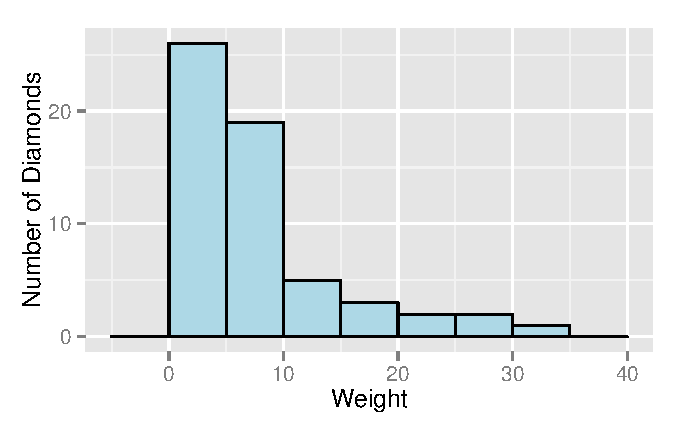
\includegraphics[scale = 0.8]{figures/ex05.pdf}
        \caption{Exercise 5}
      \end{figure}

      \begin{table}[H]
        \centering
        \begin{tabular}{rl}
          \toprule
                   & Weight \\
          \midrule
          1        & Min.   : 0.100   \\
          2        & 1st Qu.: 3.500   \\
          3        & Median : 5.400   \\
          4        & Mean   : 7.867   \\
          5        & 3rd Qu.: 9.000   \\
          6        & Max.   :33.800   \\
          \bottomrule
        \end{tabular}
      \end{table}

    \item[8]
      \begin{table}[H]
        \centering
        \begin{tabular}{rll}
          \toprule
          type    & no.outlier & with.outlier \\
          \midrule
          Min.    & 30         & 30 \\
          1st Qu. & 63         & 64 \\
          Median  & 115.0      & 117.5 \\
          Mean    & 173.3      & 225.7 \\
          3rd Qu. & 267.5      & 273.2 \\
          Max.    & 487        & 1430 \\
          SD      & 136        & 289 \\
          \bottomrule
        \end{tabular}
        \caption{Exercise 8}
      \end{table}

      \begin{figure}[H]
        \centering
        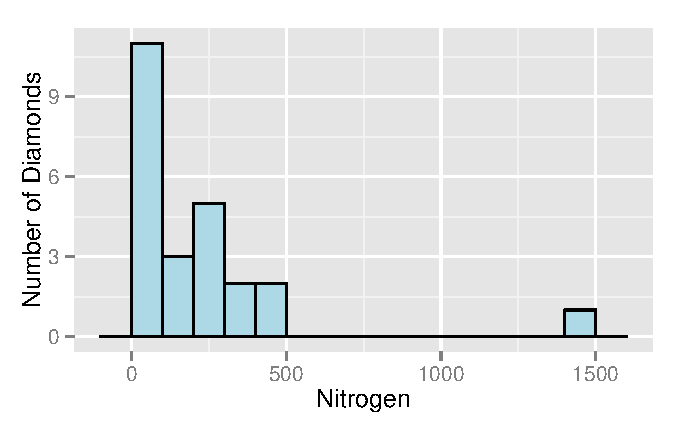
\includegraphics[scale = 0.8]{figures/ex08.pdf}
        \caption{Exercise 8}
      \end{figure}

    \item[9]
      \begin{table}[H]
        \centering
        \begin{tabular}{rll}
          \toprule
                   & Aleppo & Torrey \\
          \midrule
          Min.     & 7.2    & 21.2 \\
          1st Qu.  & 8.60   & 23.82 \\
          Median   & 9.3    & 26.7 \\
          Mean     & 9.593  & 27.000 \\
          3rd Qu.  & 10.55  & 29.70 \\
          Max.     & 12.8   & 33.7 \\
          \bottomrule
        \end{tabular}
        \caption{Exercise 9}
      \end{table}

      \begin{figure}[H]
        \centering
        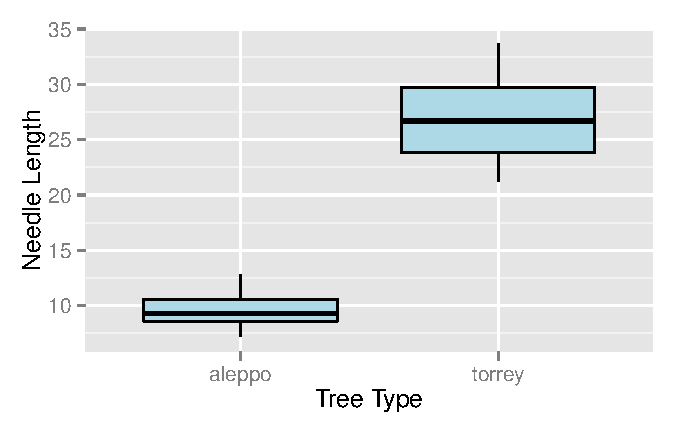
\includegraphics[scale = 0.8]{figures/ex09.pdf}
        \caption{Exercise 9}
      \end{figure}

    \item[13]
      \begin{figure}[H]
        \centering
        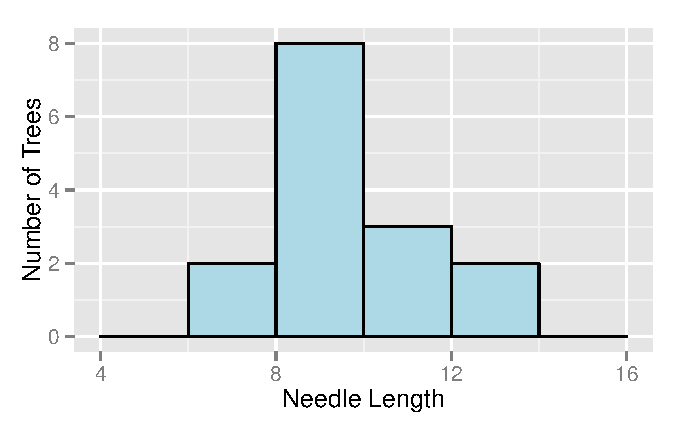
\includegraphics[scale = 0.8]{figures/ex13_aleppo.pdf}
        \caption{Exercise 13: Aleppo}
      \end{figure}

      \begin{figure}[H]
        \centering
        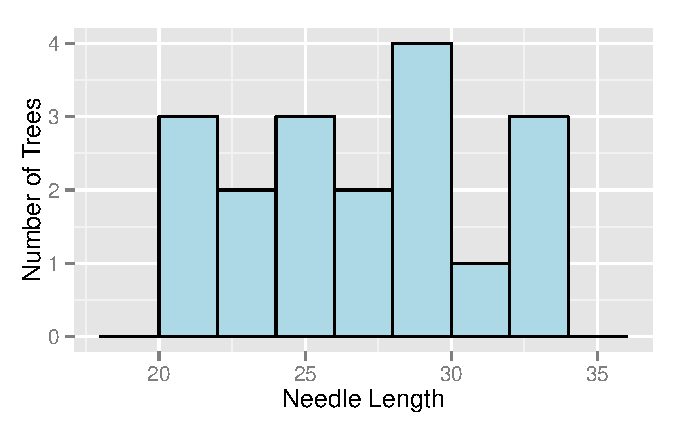
\includegraphics[scale = 0.8]{figures/ex13_torrey.pdf}
        \caption{Exercise 13: Torrey}
      \end{figure}

    \item[17]
      \begin{parts}
        \part 4.5 \% had scores higher than 13
        \part 67.3 \% had scores between 8 and 12
      \end{parts}

    \item[18]
      \begin{parts}
        \part 3.5 \% can stand 90 ksi
        \part 69 to 81 covers 25\% to 75\%
      \end{parts}

    \item[19]
      \begin{figure}[H]
        \centering
        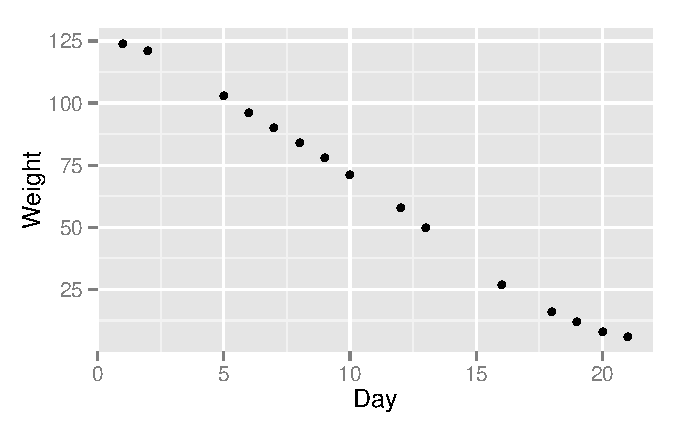
\includegraphics[scale = 0.8]{figures/ex19.pdf}
        \caption{Exercise 19}
      \end{figure}

      \begin{align*}
        r & = -0.9981 \\
        w & = 133 - 6.31 d \\
      \end{align*}

    \item[23]
      \begin{table}[H]
        \centering
        \begin{tabular}{rlrrr}
          \toprule
                   & Group & mean  & sd   & r \\
          \midrule
          1        & Lean  & 8.68  & 1.25 & 0.40 \\
          2        & Obese & 10.52 & 1.65 & 0.73 \\
          \bottomrule
        \end{tabular}
      \end{table}

      \begin{align*}
        y_l & = 0.54 + 0.083 m \\
        y_o & = 0.37 + 0.085 m \\
      \end{align*}

      \begin{figure}[H]
        \centering
        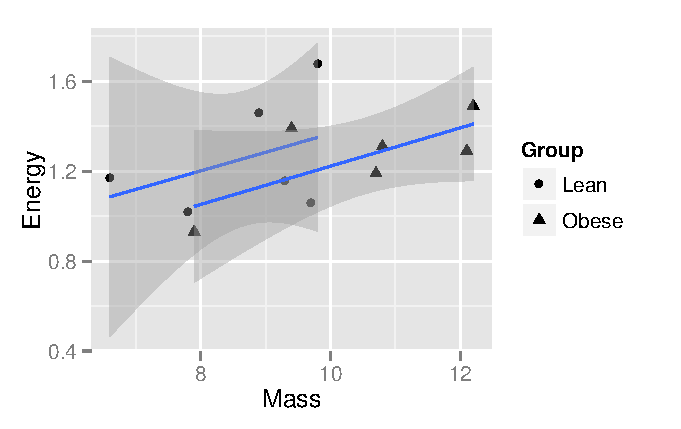
\includegraphics[scale = 0.8]{figures/ex23.pdf}
        \caption{Exercise 23}
      \end{figure}

      The slopes are the same, so the monkeys' energy use goes up at the same
      rate, regardless of lean/obese.  For a given mass, the obese monkeys use
      less energy.

    \item[24].
      \begin{table}[H]
        \centering
        \begin{tabular}{rr}
          \toprule
          mean.Smokers.      & 28.53 \\
          mean.Year.         & 1988.73 \\
          sd.Smokers.        & 6.71 \\
          sd.Year.           & 12.65 \\
          cor.Year..Smokers. & -0.98 \\
          \bottomrule
        \end{tabular}
        \caption{Exercise 24}
      \end{table}

      \[
        s  = 1066 - 0.52 y
      \]

      \begin{figure}[H]
        \centering
        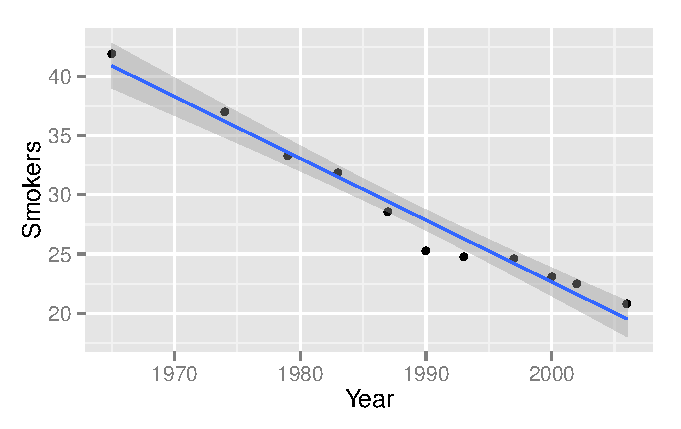
\includegraphics[scale = 0.8]{figures/ex24.pdf}
        \caption{Exercise 24}
      \end{figure}

    \item[25].
      \begin{table}[H]
        \centering
        \begin{tabular}{rr}
          \toprule
          mean.Cones.        & 1.99 \\
          mean.Offspr.       & 2.29 \\
          sd.Cones.          & 1.53 \\
          sd.Offspr.         & 0.89 \\
          cor.Cones..Offspr. & 0.76 \\
          \bottomrule
        \end{tabular}
        \caption{Exercise 25}
      \end{table}

      \[
        y = 1.4 + 0.44 x
      \]

      \begin{figure}[H]
        \centering
        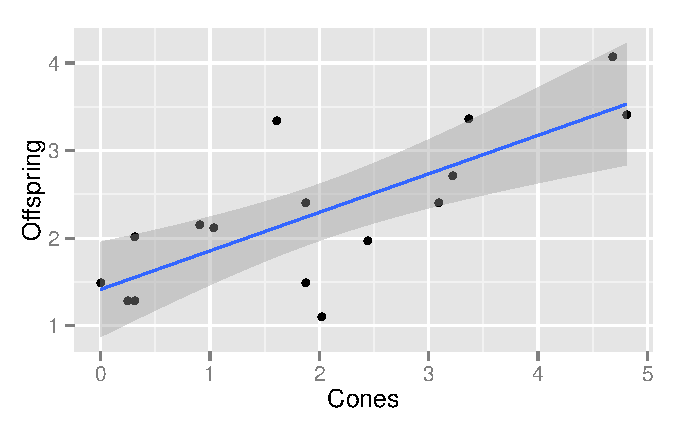
\includegraphics[scale = 0.8]{figures/ex25.pdf}
        \caption{Exercise 25}
      \end{figure}

    \item[34].
      \begin{table}[H]
        \centering
        \begin{tabular}{rlr}
          \toprule
                   & Reason & (all) \\
          \midrule
          1        & Easy   & 0.21 \\
          2        & Far    & 0.08 \\
          3        & Other  & 0.15 \\
          4        & Press  & 0.07 \\
          5        & Price  & 0.28 \\
          6        & Time   & 0.21 \\
          7        & (all)  & 1.00 \\
          \bottomrule
        \end{tabular}
      \end{table}

      \begin{table}[H]
        \centering
        \begin{tabular}{rlrr}
          \toprule
                   & Reason & Amer & Asian \\
          \midrule
          1        & Easy   & 0.24 & 0.16 \\
          2        & Far    & 0.10 & 0.06 \\
          3        & Other  & 0.17 & 0.10 \\
          4        & Press  & 0.09 & 0.04 \\
          5        & Price  & 0.15 & 0.49 \\
          6        & Time   & 0.25 & 0.14 \\
          \bottomrule
        \end{tabular}
      \end{table}

      Americans like to save time and effort while Asians like to save money.

  \end{enumerate}
\end{document}

